\documentclass[11pt]{article}
\usepackage{natbib,mybigpackage}
\usepackage{algorithm}
%\usepackage{program}
%\usepackage{algpseudocode}
\usepackage{algorithmic}
\usepackage{listings}


\def\xbf{\mathbf{x}}
\def\zbf{\mathbf{z}}
\def\xibf{\mathbf{\xi}}
\title{Documentation: Assignment 6}
\author{Abhinav Gupta\
 150123001}
\begin{document}
\titlepage
\newpage

\begin{enumerate}
\item[Q 1] Use the Box-Muller method and Marsaglia-Bray method to do the following :


(a) Generate a sample of 100, 500 and 10000 values from N(0, 1). Hence find the
sample mean and variance.


(b) Draw histogram in all cases.
\end{enumerate}

\noindent{Code for Box-Muller method (Code for 10,000 values): R}

\begin{lstlisting}
radius<-function(u){
	return (-2*log(u))
}
arg<-function(u){
	return (2*pi*u)
}
# change count to 100, 500 and 10,000 as per requirement
count<-10000
samples1<-c()
samples2<-c()
for(i in 1:count/2){
	u1<-runif(1)
	u2<-runif(1)
	samples1[i]<-sqrt(radius(u1))*cos(arg(u2))
	samples2[i]<-sqrt(radius(u1))*sin(arg(u2))
}
samples<-c(samples1,samples2)
png("question1-10000-muller.png")
hist(samples, breaks=50 ,col="light cyan",plot=TRUE)
\end{lstlisting}


\noindent{\textbf{Output}:}

Mean:  0.002538348\

Variance:  1.008891 \

\noindent{\textbf{Observation}:}
\textbf{Graph: 100 values: }\
\begin{figure}[H]
  \centering
 \subfloat[using R]{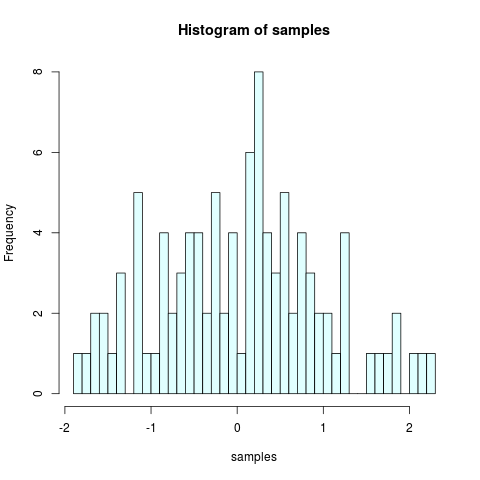
\includegraphics[width=1\textwidth]{question1-100-muller.png}}\\
\end{figure}
\textbf{Graph: 500 values: }\
\begin{figure}[H]
  \centering
 \subfloat[using R]{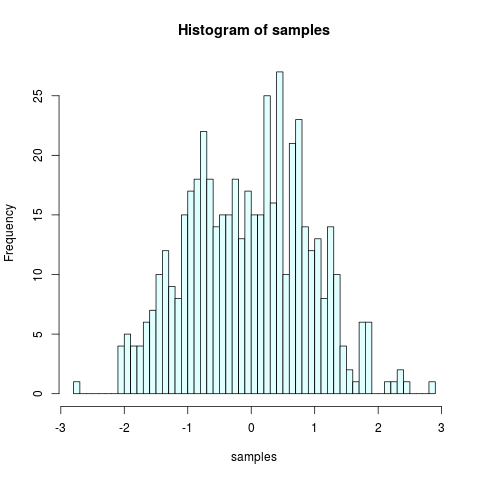
\includegraphics[width=1\textwidth]{question1-500-muller.png}}\\
\end{figure}
\textbf{Graph: 10000 values: }\
\begin{figure}[H]
  \centering
 \subfloat[using R]{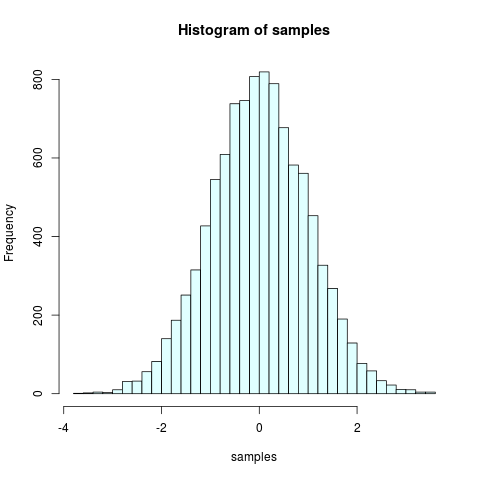
\includegraphics[width=1\textwidth]{question1-10000-muller.png}}\\
\end{figure}

\noindent{Code for Marsaglia-Bray method (Code for 10,000 values): R}

\begin{lstlisting}
square<-function(u1,u2){
	return (u1**2+u2**2)
}
intermediate<-function(x){
	return (sqrt(-2*log(x)/x))
}
# change count to 100, 500 and 10,000 as per requirement
count<-10000

samples1<-c()
samples2<-c()
i<-1
while(1){
	u1<-runif(1)
	u2<-runif(1)
	u1<-2*u1-1
	u2<-2*u2-1
	x<-square(u1,u2)
	if(x>1){
		next
	}
	y<-intermediate(x)
	samples1[i]<-u1*y
	samples2[i]<-u2*y
	i<-i+1
	count<-count-2
	if (count==0){
		break
	}
}
samples<-c(samples1,samples2)
png("question1-10000-bray.png")
hist(samples, breaks=50 ,col="light cyan",plot=TRUE)		
\end{lstlisting}


\noindent{\textbf{Output}:}

Mean:  0.009609266\

Variance:  1.006028 \

\noindent{\textbf{Observation}:}
\textbf{Graph: }\
\begin{figure}[H]
  \centering
 \subfloat[using R]{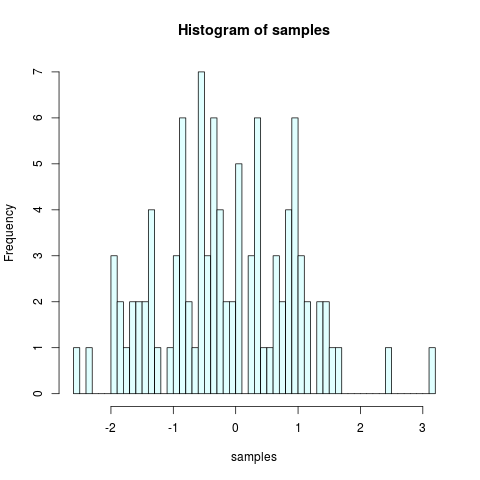
\includegraphics[width=1\textwidth]{question1-100-bray.png}}\\
\end{figure}
\textbf{Graph: 500 values: }\
\begin{figure}[H]
  \centering
 \subfloat[using R]{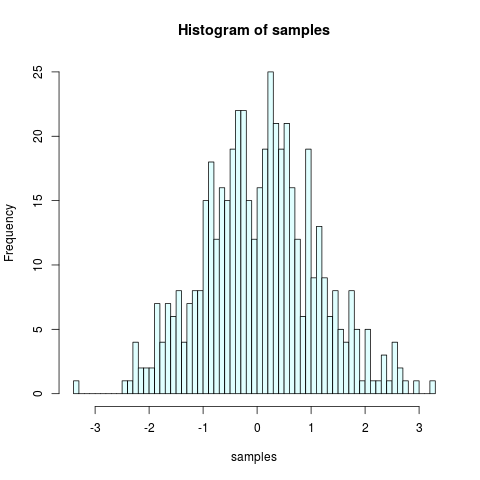
\includegraphics[width=1\textwidth]{question1-500-bray.png}}\\
\end{figure}
\textbf{Graph: 10000 values: }\
\begin{figure}[H]
  \centering
 \subfloat[using R]{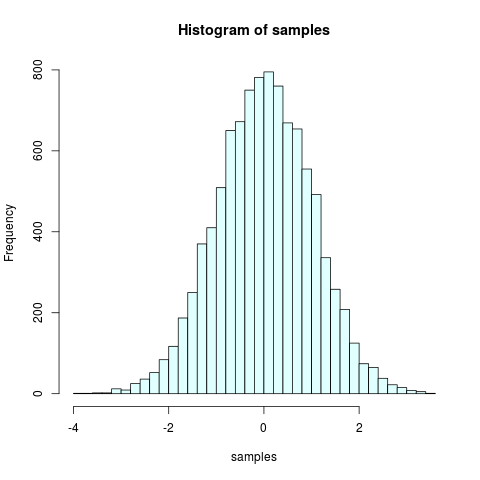
\includegraphics[width=1\textwidth]{question1-10000-bray.png}}\\
\end{figure}

%----------------------------------------------------------------------------------------------------------
\begin{enumerate}
\item[Q 2] Now use the above generated values to generated samples from N(µ = 0, σ2 = 5) and
N(µ = 5, σ2 = 5). Hence plot the empirical(from sample with size 500) distribution
function and theoretical distribution function in the same plot. (Use R/ you should
also try making the step function in C).
\end{enumerate}

\noindent{Code for Marsaglia-Bray method mean=0, variance=5 : R}
\begin{lstlisting}
square<-function(u1,u2){
	return (u1**2+u2**2)
}
intermediate<-function(x){
	return (sqrt(-2*log(x)/x))
}
count<-10000
standard_deviation<-sqrt(5)
mean<-0
samples1<-c()
samples2<-c()
i<-1
j<-0
while(1){
	u1<-runif(1)
	u2<-runif(1)
	u1<-2*u1-1
	u2<-2*u2-1
	j<-j+1
	x<-square(u1,u2)
	if(x>1){
		next
	}
	y<-intermediate(x)
	samples1[i]<-u1*y*standard_deviation+mean
	samples2[i]<-u2*y*standard_deviation+mean
	i<-i+1
	count<-count-2
	if (count==0){
		break
	}
}
samples<-c(samples1,samples2)
samples<-sort(samples)
cat("Mean is: ",mean(samples),"\n")
cat("Acceptance Probability: ",(i-1)/j,"\n")	
empirical_samples<-ecdf(samples)
png("Empirical(green).png")
plot(empirical_samples,col="green")
#par(new=TRUE)
png("Theoretical(red).png")
theoretical_samples<-pnorm(samples)
plot(theoretical_samples,col="red")
\end{lstlisting}

\begin{figure}[H]
  \centering
 \subfloat[Using R]{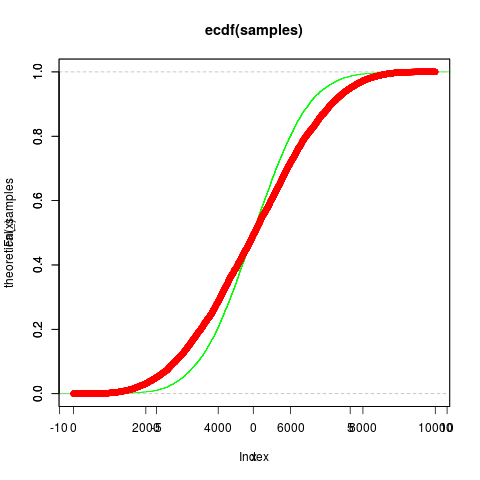
\includegraphics[width=1\textwidth]{question2-mean=0.png}}\\
\end{figure}
\begin{figure}[H]
  \centering
 \subfloat[Using R]{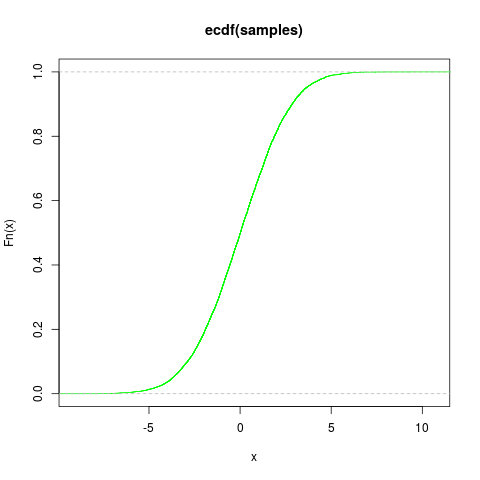
\includegraphics[width=1\textwidth]{Empirical(green).png}}\\
\end{figure}
\begin{figure}[H]
  \centering
 \subfloat[Using R]{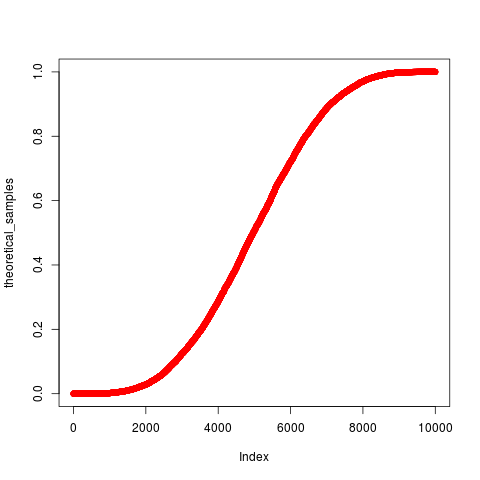
\includegraphics[width=1\textwidth]{Theoretical(red).png}}\\
\end{figure}

\noindent{Code for Marsaglia-Bray method mean=5, variance=5 : R}
\begin{lstlisting}
square<-function(u1,u2){
	return (u1**2+u2**2)
}
intermediate<-function(x){
	return (sqrt(-2*log(x)/x))
}
count<-10000
standard_deviation<-sqrt(5)
mean<-5
samples1<-c()
samples2<-c()
i<-1
j<-0
while(1){
	u1<-runif(1)
	u2<-runif(1)
	u1<-2*u1-1
	u2<-2*u2-1
	j<-j+1
	x<-square(u1,u2)
	if(x>1){
		next
	}
	y<-intermediate(x)
	samples1[i]<-u1*y*standard_deviation+mean
	samples2[i]<-u2*y*standard_deviation+mean
	i<-i+1
	count<-count-2
	if (count==0){
		break
	}
}
samples<-c(samples1,samples2)
samples<-sort(samples)
cat("Mean is: ",mean(samples),"\n")
cat("Acceptance Probability: ",(i-1)/j,"\n")	
empirical_samples<-ecdf(samples)
png("question2-mean=5.png")
plot(empirical_samples,col="green")
par(new=TRUE)
#png("Theoretical(red)--mean=5.png")
theoretical_samples<-pnorm(samples)
plot(theoretical_samples,col="red")
\end{lstlisting}

\noindent{\textbf{Observation}:}
\textbf{Graph: }\

\begin{figure}[H]
  \centering
 \subfloat[Using R]{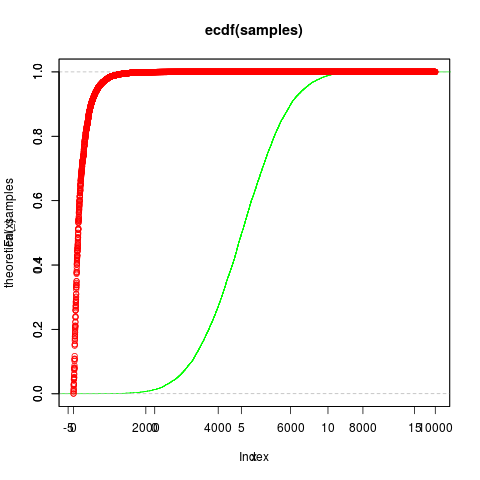
\includegraphics[width=1\textwidth]{question2-mean=5.png}}\\
\end{figure}
\begin{figure}[H]
  \centering
 \subfloat[Using R]{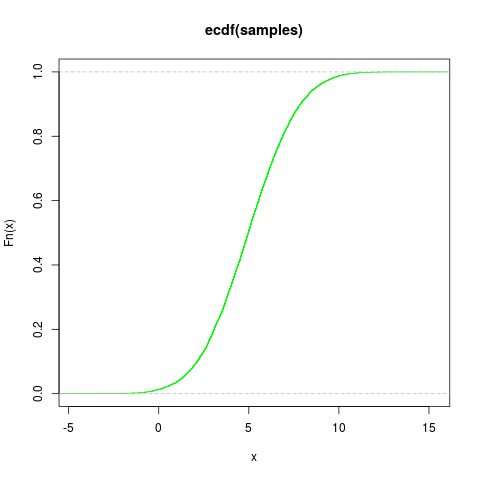
\includegraphics[width=1\textwidth]{Empirical(green)--mean=5.png}}\\
\end{figure}
\begin{figure}[H]
  \centering
 \subfloat[Using R]{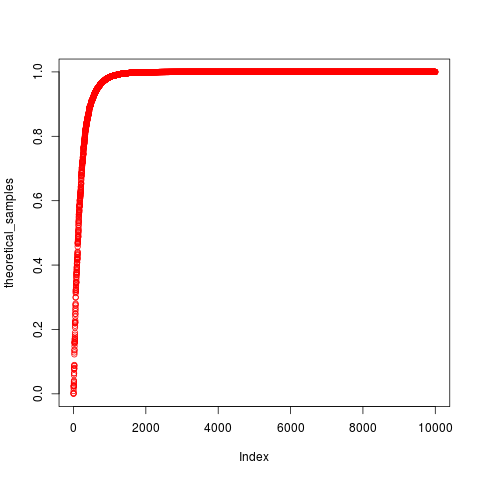
\includegraphics[width=1\textwidth]{Theoretical(red)--mean=5.png}}\\
\end{figure}

%---------------------------------------------------------------------------
\begin{enumerate}
\item[Q 3] Keep a track of the computational time required for both the methods. Which method
is faster ?
\end{enumerate}

\noindent{Code for Box-Muller method: R}

\begin{lstlisting}
radius<-function(u){
	return (-2*log(u))
}
arg<-function(u){
	return (2*pi*u)
}
count<-10000
stime<-Sys.time();
samples1<-c()
samples2<-c()
for(i in 1:count/2){
	u1<-runif(1)
	u2<-runif(1)
	samples1[i]<-sqrt(radius(u1))*cos(arg(u2))
	samples2[i]<-sqrt(radius(u1))*sin(arg(u2))
}
    

samples<-c(samples1,samples2)
etime<-Sys.time();
cat("Computation Time of Box-Muller Method: ",etime-stime,"\n");
\end{lstlisting}

\noindent{Code for Marsaglia-Bray method: R}

\begin{lstlisting}
square<-function(u1,u2){
	return (u1**2+u2**2)
}
intermediate<-function(x){
	return (sqrt(-2*log(x)/x))
}
count<-10000
stime<-Sys.time();
samples1<-c()
samples2<-c()
i<-1
while(1){
	u1<-runif(1)
	u2<-runif(1)
	u1<-2*u1-1
	u2<-2*u2-1
	x<-square(u1,u2)
	if(x>1){
		next
	}
	y<-intermediate(x)
	samples1[i]<-u1*y
	samples2[i]<-u2*y
	i<-i+1
	count<-count-2
	if (count==0){
		break
	}
}
samples<-c(samples1,samples2)
etime<-Sys.time();
cat("Computation Time of Marsaglia-Bray Method: ",etime-stime,"\n");
\end{lstlisting}


\noindent{\textbf{Output}:}

\textbf{Computation Time of Box-Muller Method:  0.1807923}\

\textbf{Computation Time of Marsaglia-Bray Method:  0.1370828}\

%---------------------------------------------------------------------------
\begin{enumerate}
\item[Q 4] For the Marsaglia-Bray method keep track of the proportional of values rejected. How
does it compare with 1 −pi/4 ??
?
\end{enumerate}
\noindent{Code for Marsaglia-Bray method: R}

\begin{lstlisting}
square<-function(u1,u2){
	return (u1**2+u2**2)
}
intermediate<-function(x){
	return (sqrt(-2*log(x)/x))
}
count<-1000
ap<-c()
for(k in 1:20){
samples1<-c()
samples2<-c()
i<-1
j<-0
while(1){
	u1<-runif(1)
	u2<-runif(1)
	u1<-2*u1-1
	u2<-2*u2-1
	j<-j+1
	x<-square(u1,u2)
	if(x>1){
		next
	}
	y<-intermediate(x)
	samples1[i]<-u1*y
	samples2[i]<-u2*y
	i<-i+1
	count<-count-2
	if (count==0){
		break
	}
}
count<-count+1000
ap[k]<-(((i-1)/j)/(1-pi/4))
}
samples<-c(samples1,samples2)
k<-1
test<-c()
constant<-1000
for (k in 1:20){
	test[k]<-constant*k
}
cat("Acceptance Probability: ",(i-1)/j,"\n")	
plot(test,ap,type="l",col="red")	
\end{lstlisting}

\noindent{\textbf{Observation}:}
\textbf{Graph: }\

\begin{figure}[H]
  \centering
 \subfloat[Using R]{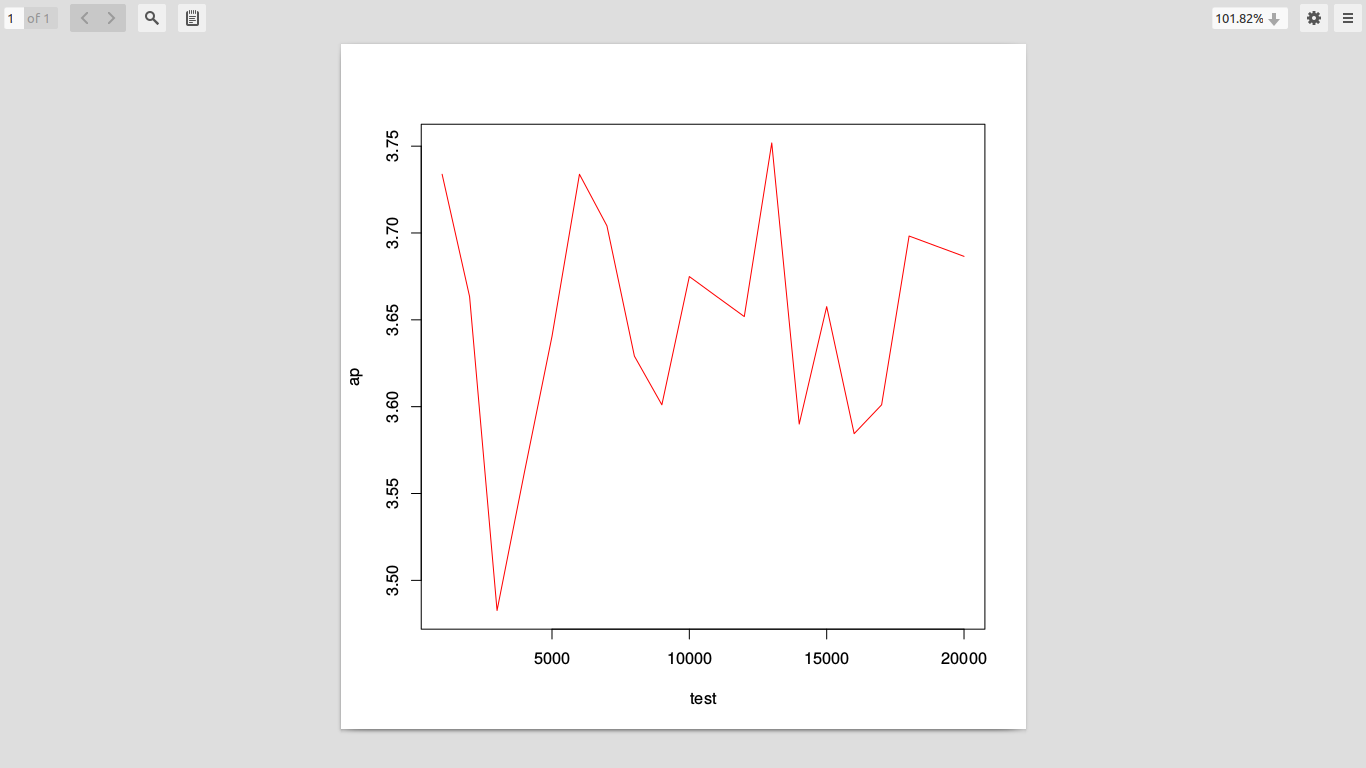
\includegraphics[width=1\textwidth]{acceptance by 1-pi divide 2.png}}\\
\end{figure}

\end{document}
